%% bare_jrnl.tex
%% V1.4b
%% 2015/08/26
%% by Michael Shell
%% see http://www.michaelshell.org/
%% for current contact information.
%%
%% This is a skeleton file demonstrating the use of IEEEtran.cls
%% (requires IEEEtran.cls version 1.8b or later) with an IEEE
%% journal paper.
%%

\documentclass[journal,onecolumn]{IEEEtran}
%
% If IEEEtran.cls has not been installed into the LaTeX system files,
% manually specify the path to it like:
% \documentclass[journal]{../sty/IEEEtran}

\usepackage[pdftex]{graphicx}
\usepackage{amsmath}
\usepackage{amssymb}
\usepackage{algpseudocode}
\usepackage{algorithm}
\usepackage{xpatch}
\usepackage{cite}
\usepackage{tikz}
\usetikzlibrary{shapes, arrows}

%\usepackage{array}
%\usepackage[caption=false,font=normalsize,labelfont=sf,textfont=sf]{subfig}
%\usepackage{url}

\hyphenation{op-tical net-works semi-conduc-tor}

%% For algorithms...
\algrenewcommand\alglinenumber[1]{{\sffamily\footnotesize#1:}}
\makeatletter
\xpatchcmd{\algorithmic}{\itemsep\z@}{\itemsep=5pt}{}{}
\makeatother
\renewcommand{\algorithmicrequire}{\textbf{Input:}}
\renewcommand{\algorithmicensure}{\textbf{Output:}}
\renewcommand{\algorithmicforall}{\textbf{For Each}}

% Define block styles for tikz...
\tikzstyle{decision} = [diamond, draw, fill=blue!20, text width=4.5em, 
    text centered, node distance=3cm, inner sep=0pt]
\tikzstyle{block} = [rectangle, draw, fill=blue!20, text width=3cm, 
    text centered, rounded corners, minimum height=4em]
\tikzstyle{info} = [rectangle, scale=0.9, text width=5cm, minimum height=4em, node distance=4.75cm]
\tikzstyle{line} = [draw, -latex']
\tikzstyle{cloud} = [draw, ellipse,fill=red!20, node distance=3cm,
    minimum height=2em]
\tikzstyle{io} = [trapezium, trapezium left angle=70, trapezium right angle=110, 
    minimum height=1cm, text centered, draw=black, fill=blue!30]

\begin{document}
% \title{_}
% \author{_}
% 
% \maketitle

\section{Methods}
%\IEEEPARstart{T}{his} 
This section explains two alternative methodologies to find moving flock patterns in large spatio-temporal datasets using modern distributed frameworks to divide and parallelize the work load but,  before to explain the details of our contributions, we will explains the in a genaral manner the details of the current state-of-the-art to highlight the challenges and drawbacks at the moment to dealt with very large spatio-temporal datasets.

\subsection{The BFE algorithm}
The alternatives we will discuss later follows closely the steps explained at \cite{vieira_2009}.  In this work, the authors proposed the Basic Flock Evaluation (BFE) algorithm to find flock patterns on trajectory databases.  The details of the algorithm can be accessed at the source but we will explaing the main aspects in a general view.  It is important to clarify that BFE runs in two phases: firstly, it finds valid disks in the current time instant; secondly, it combines previous flocks with the recently discovered disks to extend them and report them.  

The main inputs of the BFE algorithm are a set of points, a minimum distance $\varepsilon$ which will define the diameter of the disks where the moving entities should lay, a minimum number of entities $\mu$ at each disk and a minimum duration $\delta$ which is the minumun number of time units the entities should be keep together to be considered a flock.  Based on these inputs,  figure \ref{fig:MF_flowchart} breaks down schematically the work flow  of this phase where we can identify 4 general steps.  The main goal of this phase is to find a set of valid disks at each time instant to allow further combinations with subsequents set of disks coming in the future.

\begin{figure}[!ht]
    \centering
    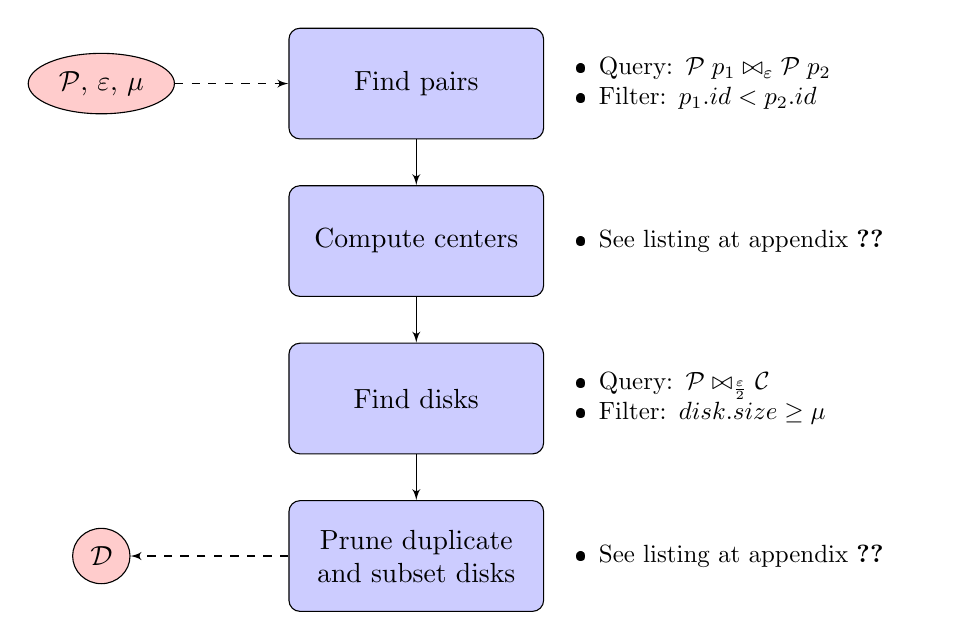
\begin{tikzpicture}[node distance = 2cm, auto]
        % Place nodes
        \node [block] (pairs) {Find pairs};
        \node [cloud, node distance=4cm, left of=pairs] (input) {$\mathcal{P}$, $\varepsilon$, $\mu$};
        \node [block, below of=pairs] (centers) {Compute centers};
        \node [block, below of=centers] (disks) {Find disks};
        \node [block, below of=disks] (maximals) {Prune duplicate and subset disks};
        \node [cloud, node distance=4cm, left of=maximals] (output) {$\mathcal{D}$};
        % Info nodes
         \node [info, right of=pairs] (pairs_info) {
            \textbullet \hspace{0.1em} Query: $\mathcal{P}\;p_1 \bowtie_{\varepsilon} \mathcal{P}\;p_2$ \\
            \textbullet \hspace{0.1em} Filter: $p_1.id < p_2.id$ 
         };
        \node [info, right of=centers] (centers_info) { 
            \textbullet \hspace{0.1em} See listing at appendix \ref{app:centers}
        };
        \node [info, right of=disks] (disks_info) {
            \textbullet \hspace{0.1em} Query: $\mathcal{P} \bowtie_{\frac{\varepsilon}{2}} \mathcal{C}$ \\
            \textbullet \hspace{0.1em} Filter: $disk.size \geq \mu $ 
         };
        \node [info, right of=maximals] (maximals_info) { 
            \textbullet \hspace{0.1em} See listing at appendix \ref{app:disks} 
        };
        % Draw edges
        \path [line,dashed] (input) -- (pairs);
        \path [line] (pairs) -- (centers);
        \path [line] (centers) -- (disks);
        \path [line] (disks) -- (maximals);
        \path [line,dashed] (maximals) -- (output);
    \end{tikzpicture}
    
    \caption{General steps in phase 1 of the BFE algorithm.}\label{fig:MF_flowchart}
\end{figure}

The main steps in phase one can are explained as follows:
\begin{enumerate}
    \item Pair finding:  Using the $\varepsilon$ parameter, the algorithm query the set of points to get the set of pairs which laid at a maximum distance of $\varepsilon$ units.  Usually, it is a distance self-join operation over the set of points using $\varepsilon$ as the distance parameter.  The query also pays attention to do not return pair duplicates.  For instance, the pair between point $p_1$ and $p_2$ is the same that pair between $p_2$ and $p_1$ and just one of them should be reported (the id of each point is used to filter duplicates).
    \item Center computation:  From the previous set of pairs, each tuple is the input of a simple computation to locate the centers of the two circles of radius $\frac{\varepsilon}{2}$ which circumference laid on the input points.  The pseudocode of the procedure can be seen in appendix \ref{app:centers}.
    \item Disk finding: Once the centers have been identified, a query to collect the points around those centers is needed in order to group the set of points which laid $\varepsilon$ distance units each other.  This is done by running a distance join query between the set of points and the set of centers using $\frac{\varepsilon}{2}$ as the distance parameter. Therefore, a disk will be defined by its center and the IDs of the points around it. At this stage, a filter is applied to remove those disks which collect less than $\mu$ entities around it.
    \item Disk pruning: It is possible than a disk collects the same set of points, or a subset, of the set of points of another disk.  In such cases the algorithm should report just that one which contains the others.  An explanation of the procedure can be seen in appendix \ref{app:disks}.
\end{enumerate}

It is important to note that BFE also proposes a grid index structure in this phase to speed up spatial operations.  The algorithm divides the space area in a grid of $\varepsilon$ side (see figure \ref{fig:grid} from \cite{vieira_2009}).  In this way, BFE just processes each grid and its 8 neighbor grids.  It does not need to query grids outside of its neighborhood given that points in other grids are far away to affect the results.

\begin{figure}
    \centering
    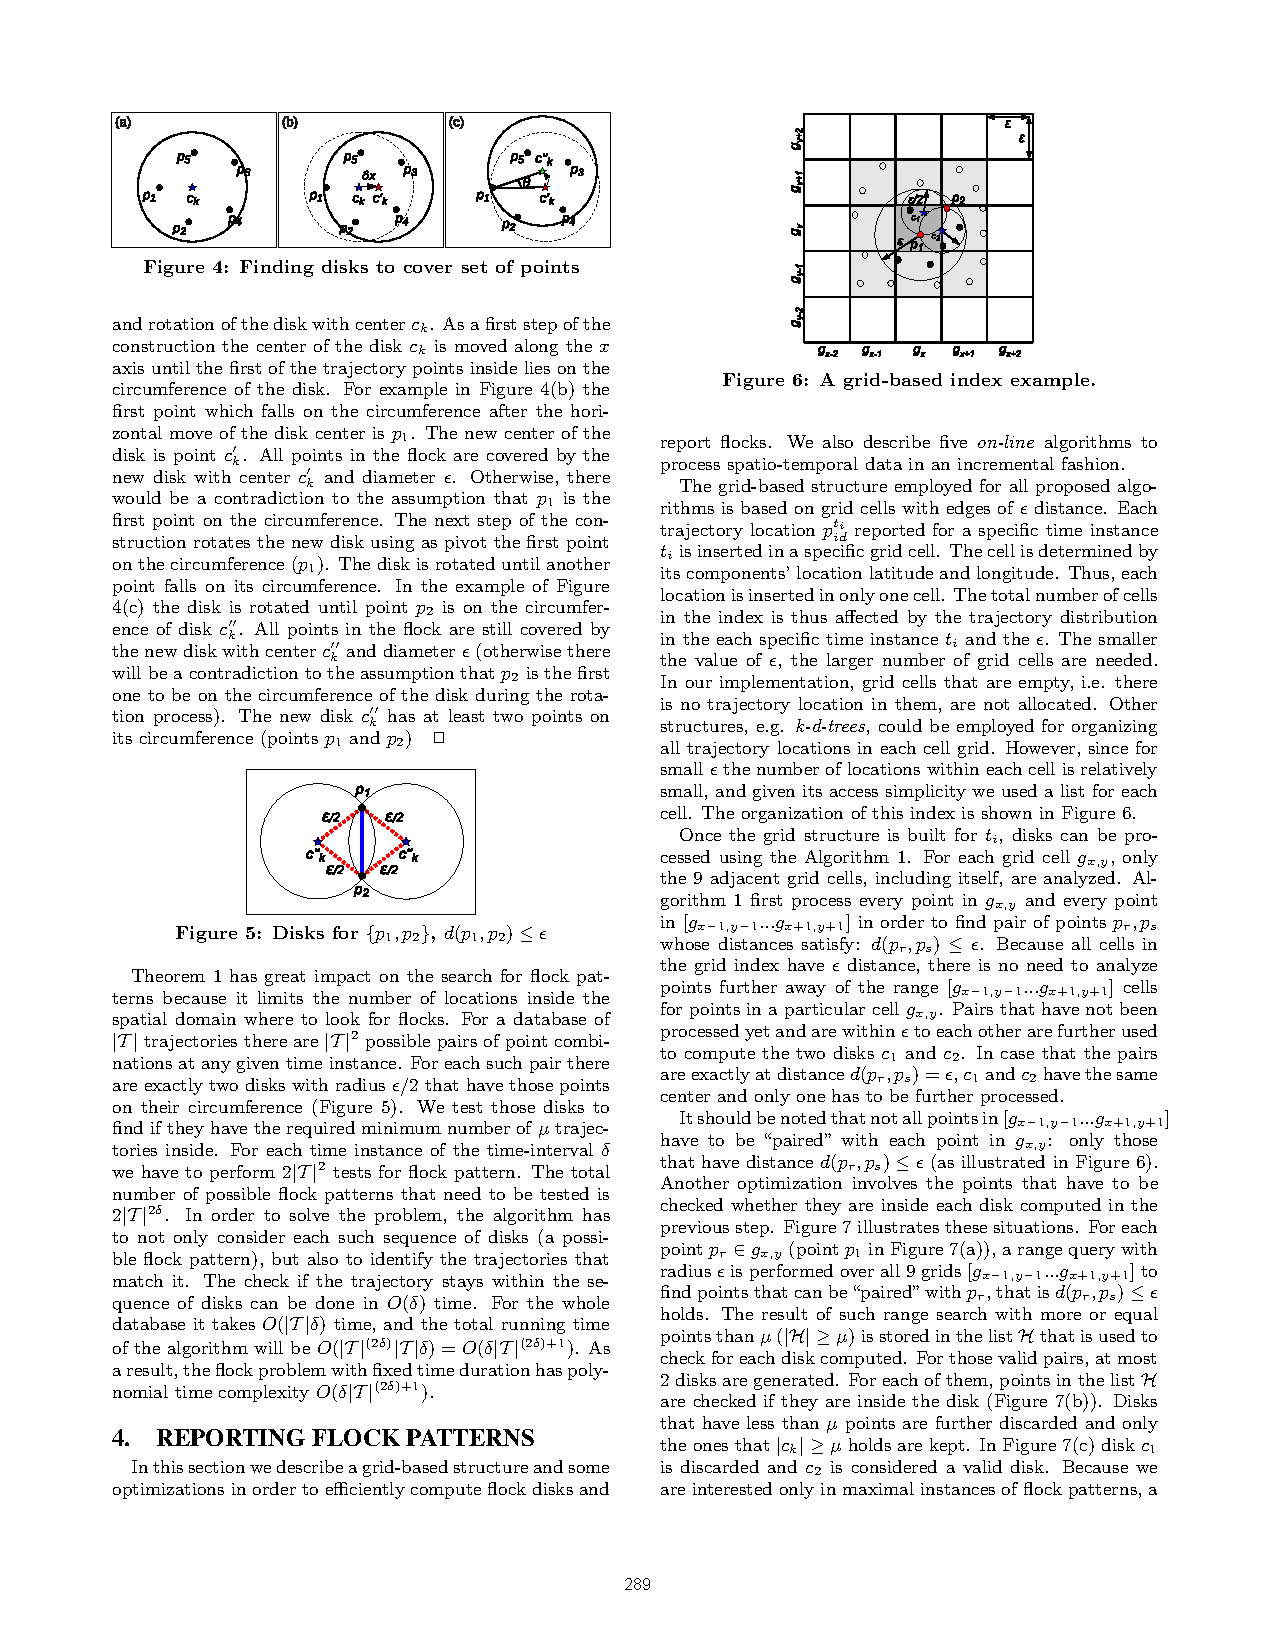
\includegraphics[clip,trim=13cm 21.75cm 4.1cm 1.85cm]{figures/grid}
    \caption{The grid-based index structure proposed at \cite{vieira_2009}.}\label{fig:grid}
\end{figure}

The second phase is more straighforward.  Figure \ref{fig:FF_flowchart} explains schematically what is done once the set of current disks (as explained in figure \ref{fig:MF_flowchart}) is found at every time instant.  This phase performs a recursion using the current set of disks and the previous set of flocks which comes from the  previous time instant.  Due to we do not know where and how far a group of entities can move in the next time instant, a cross product between both sets is requiered.  

\begin{figure}[!ht]
    \centering
    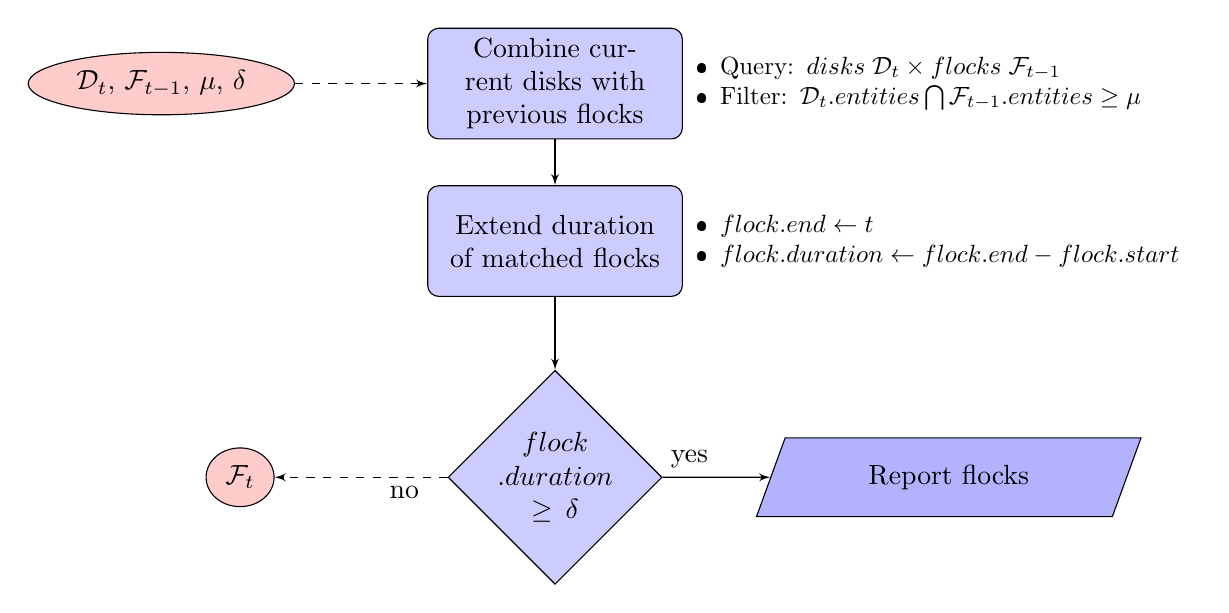
\begin{tikzpicture}[node distance = 2cm, auto]
        % Place nodes
        \node [block] (combine) {Combine current disks with previous flocks};
        \node [cloud, left of=combine, node distance=5cm] (input) 
            {$\mathcal{D}_t$, $\mathcal{F}_{t-1}$, $\mu$, $\delta$};
        \node [block, below of=combine] (extend) {Extend duration of matched flocks};
        \node [decision, below of=extend] (decide) {$flock$\\$.duration$\\$\geq \delta$};
        \node [io, right of=decide, node distance=5cm] (report) {Report flocks};
        \node [cloud, left of=decide, node distance=4cm] (output) {$\mathcal{F}_t$};
        % Info nodes
         \node [info, right of=combine, node distance=5.5cm, text width=7cm] (combine_info) {
            \textbullet \hspace{0.1em} Query: $disks\;\mathcal{D}_t \times flocks\;\mathcal{F}_{t-1}$ \\
            \textbullet \hspace{0.1em} Filter: $\mathcal{D}_{t}.entities \bigcap \mathcal{F}_{t-1}.entities \geq \mu$ 
         };
         \node [info, right of=extend, node distance=5.5cm, text width=7cm] (extend_info) {
            \textbullet \hspace{0.1em} $flock.end \gets t$ \\
            \textbullet \hspace{0.1em} $flock.duration \gets flock.end - flock.start$ 
         };        
         % Draw edges
        \path [line,dashed] (input) -- (combine);
        \path [line] (combine) -- (extend);
        \path [line] (extend) -- (decide);
        \path [line] (decide) -- node [near start] {yes} (report);
        \path [line, dashed] (decide) -- node [near start] {no}  (output);
    \end{tikzpicture}
    \caption{Steps in BFE phase two. Combination, extension and reporting of flocks.}\label{fig:FF_flowchart}
\end{figure}

However, just disks which match the entities of previous flocks are kept.  Indeed, only when the size of common items is greater than $\mu$ we keep the pair.  Then, it updates the end time and duration of the filtered flocks.  This information is used to decide if it is time to report a flock or keep it for further analysis.  If the duration has reached the minimum duration $\delta$, a flock is reported and removed from the set.  The remaining flocks are sent to the next iteration for further evaluation in the next time instant.

Similarly, figure \ref{fig:FF_stages} illustrates the recursion and how the set of flocks from previous time instants feeds the next iteration.  The example asumes a $\delta$ value of 3, so it starts reporting flock since time instant $t_2$.  Note that time instants $t_0$ and $t_1$ are initial conditions.  At the very begining of the execution, we just can find valid disks at $t_0$ which inmediately are tranformed to flocks of duration 1 and feed the next time instant.  At $t_1$ we can find a new set of disks $\mathcal{D}_1$ which combines with the set of previous flocks $\mathcal{F}_0$.  It updates the information of each flock accordingly but it does not report any flock yet.  From now on, subsequent time instants follows strictly the steps summarized on figure \ref{fig:FF_flowchart}.

\begin{figure}[!ht]
    \centering
    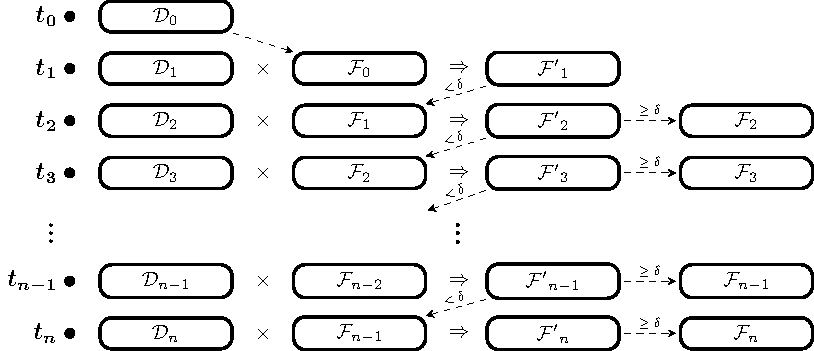
\includegraphics[width=0.75\textwidth]{figures/FF_stages}
    \caption{BFE phase 2 example explaining the recursion of the set of flocks along time instants and the initial conditions.}\label{fig:FF_stages}
\end{figure}

\subsection{Bottlenecks in BFE and possible solutions}
There are some steps during the execution of BFE which are particularly affected when it deals with very large datasets.  Firstly, we will focus on phase 1 of BFE.  Figure \ref{fig:example}, the steps of this phase are illustrated for a sample dataset.  You can see that the number of centers and disks found is considerable large in comparisson with the final set of valid disks.  Indeed, the finding of centers and posterior operations grows exponentially depending on the number of points and possible pairs (which itself depend on the $\varepsilon$ paramenter).   

\begin{figure}[!ht]
    \centering
    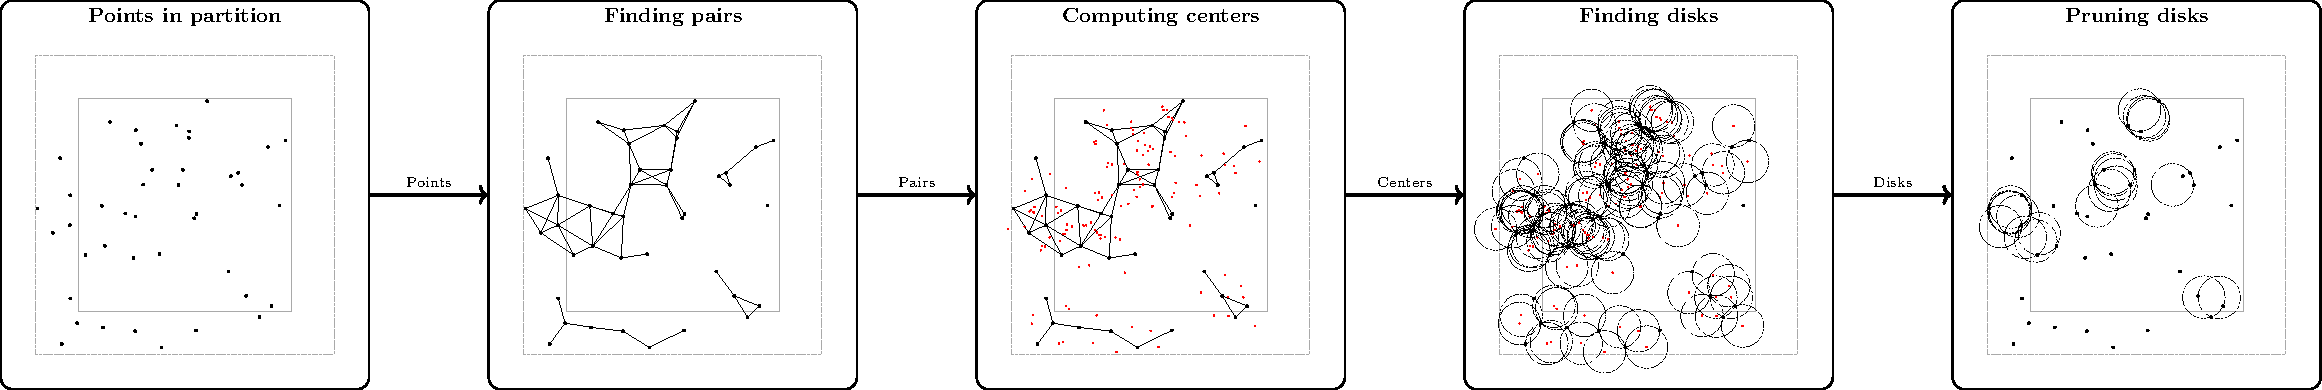
\includegraphics[width=1\textwidth]{figures/MF_stages/flow}
    \caption{Example of BFE execution on a sample dataset..}\label{fig:example}
\end{figure}

\subsection{A parallel approach}
\begin{figure}[!ht]
    \centering
    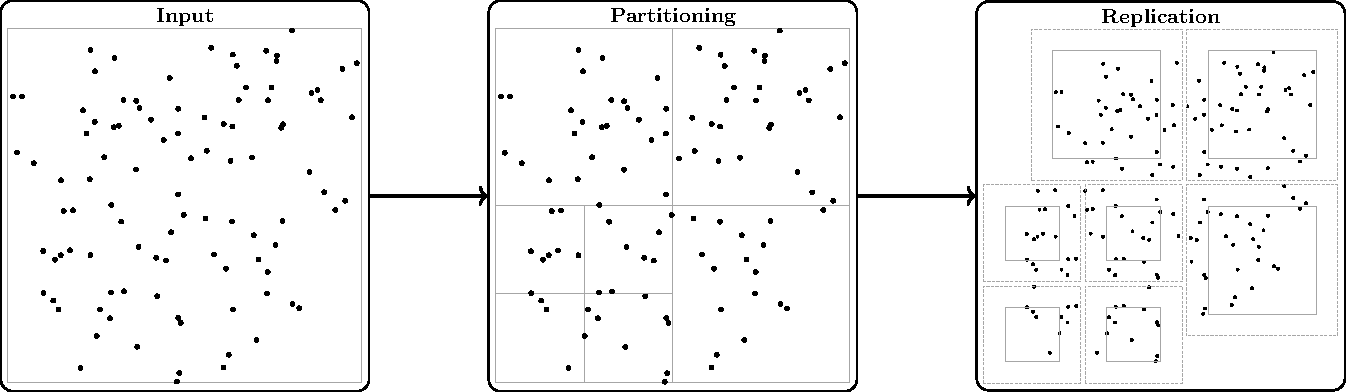
\includegraphics[width=\textwidth]{figures/MF_stages/P123}
    \caption{An example of partitioning and replication on a sample dataset.}\label{fig:partrep}
\end{figure}


\newpage 

\appendices
\section{Center computation.}\label{app:centers}

\alglanguage{pseudocode}
\begin{algorithm}
    \caption{Find the centers of given radius which circumference laid on the two input points.}
    \begin{algorithmic}[1]
        \Require Radius $\frac{\varepsilon}{2}$ and points $p_1$ and $p_2$.
        \Ensure Centers $c_1$ and $c_2$.
        
        \Function{FindCenters}{$p_1$, $p_2$, $\frac{\varepsilon}{2}$}
        \State $r^2 \gets (\frac{\varepsilon}{2})^2$
        \State $X \gets p_1.x - p_2.x$
        \State $Y \gets p_1.y - p_2.y$
        \State $d^2 \gets X^2 + Y^2$
        \State $R \gets \sqrt{\lvert 4 \times \frac{r^2}{d^2} - 1 \rvert}$
        \State $c_1.x \gets X + \frac{Y \times R}{2} + p_2.x$
        \State $c_1.y \gets Y - \frac{X \times R}{2} + p_2.y$
        \State $c_2.x \gets X - \frac{Y \times R}{2} + p_2.x$
        \State $c_2.y \gets Y + \frac{X \times R}{2} + p_2.y$
        
        \State \Return $c_1$ and $c_2$
        \EndFunction
    \end{algorithmic}
\end{algorithm}

\newpage

\section{Disk pruning.}\label{app:disks}

\begin{algorithm}
    \caption{Prune disks which are duplicate or subset of others.}
    \begin{algorithmic}[1]
        \Require Set of disks $D$.
        \Ensure Set of disks $D^{\prime}$ without duplicate or subsets.
        
        \Function{pruneDisks}{$D$}
        \State $E \gets \varnothing$
        \ForAll{disk $d_i$ in $D$}
            \State $N \gets d_i \cap D$
            \ForAll{disk $n_j$ in $N$}
                \If{$d_i$ contains all the elements of $n_j$}
                        \State $E \gets E \cup {n_j}$
                \EndIf
            \EndFor
        \EndFor        
        \State $D^{\prime} \gets D \setminus E$
        \State \Return $D^{\prime}$
        \EndFunction
    \end{algorithmic}
\end{algorithm}

\bibliographystyle{IEEEtran}
\bibliography{../pflocks.bib}

\end{document}
